\documentclass[aspectratio=169,usenames,dvipsnames,pdftex]{beamer}

\usepackage{listings}
\usepackage{xcolor}
\usepackage{multicol}
\usepackage{media9}
\usepackage{siunitx}
\usepackage[scale=2]{ccicons}
\usepackage{caption}
\usepackage{subcaption}
\usepackage{tabularx}
\usepackage{lmodern}
\usepackage{anyfontsize}
\usepackage{fontawesome5}
\usepackage{booktabs}
\usepackage{appendixnumberbeamer}
\usepackage{csquotes}
\usepackage{pgfplots}
\usepgfplotslibrary{dateplot}
\usepackage{tikz}
\usetikzlibrary[topaths]
\usepackage{xspace}
\usetikzlibrary{shapes,snakes}
\usepackage{amsmath,amssymb}

\graphicspath{{resources/}}


%%%%%%%%%%%%%%%%
%% Title Page %%
%%%%%%%%%%%%%%%%
\title{Devault (graduation project)}
\subtitle{\texttt{A Blockchain-based end-to-end encrypted cloud storage}}
\date {}
\author {}
\institute {
  \begin{multicols}{2}
    \begin{flushleft}
      \texttt{Participants:} \\
      \texttt{\large{Abd El-Twab M. Fakhry}} \\
      \texttt{\large{Hossam A. Eissa}}
    \end{flushleft}
    \begin{flushleft}
      \texttt{Supervisor:} \\
      \texttt{\large{Dr. Abdurrahman Nasr}}
    \end{flushleft}
  \end{multicols}

  \centering
  \scshape{Al-Azhar University} \\
  \scshape{\small Faculty of Engineering} \\
  \scshape{\normalsize Computers \& Systems Engineering Department} \\\vspace{8pt}
  \today
}

\titlegraphic{\hfill
\includegraphics[height=1.5cm]{devault-1024.png}}

%%%%%%%%%%%%%%%%%%%
%% Common colors %%
%%%%%%%%%%%%%%%%%%%
\definecolor{charcoal}{rgb}{0.21, 0.27, 0.31}
\definecolor{champagne}{rgb}{0.97, 0.91, 0.81}
\definecolor{dimgray}{rgb}{0.41, 0.41, 0.41}
\definecolor{flax}{rgb}{0.93, 0.86, 0.51}
%% Code colors
\definecolor{lavendergray}{rgb}{0.77, 0.76, 0.82}
\definecolor{lightslategray}{rgb}{0.47, 0.53, 0.6}
\definecolor{egyptianblue}{rgb}{0.06, 0.2, 0.65}
\definecolor{ballblue}{rgb}{0.13, 0.67, 0.8}
\definecolor{greencssgreen}{rgb}{0.0, 0.5, 0.0}
\definecolor{eggshell}{rgb}{0.94, 0.92, 0.84}
\definecolor{lava}{rgb}{0.81, 0.06, 0.13}
\definecolor{lavenderindigo}{rgb}{0.58, 0.34, 0.92}
\definecolor{mediumred-violet}{rgb}{0.73, 0.2, 0.52}
\definecolor{black}{rgb}{0.0, 0.0, 0.0}
\definecolor{forestgreen}{rgb}{0.13, 0.55, 0.13}
\definecolor{harvardcrimson}{rgb}{0.79, 0.0, 0.09}

%%%%%%%%%%%%%%%%%%%%%%%%%
%% Syntax Highlighting %%
%%%%%%%%%%%%%%%%%%%%%%%%%
\lstdefinestyle{shared} {
  tabsize=2,
	showtabs=false,
	keepspaces=true,
  breaklines=true,
  showspaces=false,
  showstringspaces=false,
	breakatwhitespace=false,
  belowcaptionskip=1\baselineskip,
	captionpos=b,
  xleftmargin=\parindent,
	basicstyle=\ttfamily\footnotesize,
  numbers=left,
  numbersep=6pt,
	numberstyle=\tiny\color{lavenderindigo},
}

\lstdefinestyle{c}{
	language=C,
  style=shared,
	backgroundcolor=\color{eggshell},
	keywordstyle=\bfseries\color{egyptianblue},
	commentstyle=\itshape\color{lava},
  morecomment=[s][\color{forestgreen}]{/*+}{*/},
  morecomment=[s][\color{harvardcrimson}]{/*-}{*/},
	stringstyle=\color{greencssgreen},
	numberstyle=\tiny\color{lavenderindigo},
  % identifierstyle=\color{black},
  otherkeywords={size, printf, scanf, sizeof, memset},
  alsoletter = {\#},
  keywords=[2]{\#if,\#endif,\#else},
}

\lstdefinestyle{cpp} {
  language=C++,
  style=shared,
	backgroundcolor=\color{eggshell},
	keywordstyle=\bfseries\color{egyptianblue},
	commentstyle=\itshape\color{lava},
  morecomment=[s][\color{forestgreen}]{/*+}{*/},
  morecomment=[s][\color{harvardcrimson}]{/*-}{*/},
	stringstyle=\color{greencssgreen},
	numberstyle=\tiny\color{lavenderindigo},
  % identifierstyle=\color{black},
  otherkeywords={size, front, back, cin, cout, endl, sizeof, memset},
  alsoletter = {\#},
  keywords=[2]{\#if,\#endif,\#else},
}

\lstdefinelanguage{solidity} {
  morekeywords={pragma, contract, address, uint, bool, event, public,
    payable, constructor, function, require, for, if, emit, return,
    true, false, memory, storage},
  sensitive=true,
  morecomment=[l]{//},
  morecomment=[s]{/*}{*/},
  morecomment=[s][\color{forestgreen}]{/*+}{*/},
  morecomment=[s][\color{harvardcrimson}]{/*-}{*/},
  morestring=[b]",
  morestring=[b]'
}

\lstdefinestyle{solidity} {
  style=shared,
  language=solidity,
	backgroundcolor=\color{eggshell},
	keywordstyle=\bfseries\color{egyptianblue},
	commentstyle=\itshape\color{lava},
	stringstyle=\color{greencssgreen},
	numberstyle=\tiny\color{lavenderindigo},
  % identifierstyle=\color{black},
  otherkeywords={},
}


%%%%%%%%%%%
%% Theme %%
%%%%%%%%%%%
\usetheme[
progressbar=frametitle,
titleformat=smallcaps,
numbering=fraction,
block=fill,
background=light
]{metropolis}

\useoutertheme{metropolis}
\useinnertheme{metropolis}
\usefonttheme{metropolis}
\usecolortheme{seahorse}
\setbeamercolor{background canvas}{bg=champagne}
\setbeamercovered{transparent=5}

%%%%%%%%%%%%%%%%%%%%%%
%% Global Variables %%
%%%%%%%%%%%%%%%%%%%%%%
\newcommand{\themename}{\textbf{\textsc{Metropolis}}\xspace}
\newcommand{\Item}[1]{\texttt{\textbf{#1}}}

%%%%%%%%%%%%%%%%%%%%
%% Document Start %%
%%%%%%%%%%%%%%%%%%%%
\begin{document}

	\maketitle

	\begin{frame}{Table of contents}
		\setbeamertemplate{section in toc}[sections numbered]
		\tableofcontents[hideallsubsections]
	\end{frame}

  \section{{Introduction}}

  \begin{frame}[t]{Background and Motivation}\vspace{8pt}
    \scshape{\Large What is Web 1.0?} \\[4pt]
    \normalshape{}
    Basically, this first version of the web was designed to help people better find information. This web version dealt was dedicated to users searching for data. This web version is sometimes called \textit{``the read-only Web''} because it lacks the necessary forms, visuals, controls, and interactivity we enjoy on today’s Internet.

    \begin{itemize}
    \item No user-to-server communication.
    \item Static websites.
    \item Hyper-linking and bookmarking pages.
    \item Read-only Web.
    \end{itemize}

    \textit{\texttt{\textcolor{RoyalBlue}{Active 1989-2005}}}
  \end{frame}

  \begin{frame}[t]{Background and Motivation}\vspace{8pt}
    \scshape{\Large What is Web 2.0?} \\[4pt]
    \normalshape{}
    If Web 1.0 was made up of a small number of people generating content for a larger audience, then Web 2.0 is many people creating even more content for a growing audience. Web 1.0 focused on reading; Web 2.0 focused on participating and contributing.

    \begin{itemize}
    \item Functions such as online documents, video streaming, etc.
    \item Cloud computing operations
    \item Centralized data.
    \item Read and Write Web.
    \end{itemize}

    \textit{\texttt{\textcolor{RoyalBlue}{Active 1999-2012}}}
  \end{frame}

  \begin{frame}[t]{Background and Motivation}\vspace{8pt}
    \scshape{\Large What is Web 3.0?} \\[4pt]
    \normalshape{}
    Web 3.0, which is also referred to as Web3, is built on a foundation consisting of the core ideas of decentralization, openness, and more excellent user utility. Web 1.0 is the ``read-only Web,'' Web 2.0 is the ``participative social Web,'' and Web 3.0 is the ``read, write, execute Web.''

    \begin{itemize}
    \item The Internet of Things (IoT).
    \item Semantic searches.
    \item Decentralized processes.
    \item Read, Write, and Control Web.
    \end{itemize}

    \textit{\texttt{\textcolor{RoyalBlue}{Active 2006-ongoing}}}
  \end{frame}

  \begin{frame}[t]{Problem Statement}
    \scshape{\Large What is wrong?}
    \normalshape{}

    \begin{itemize}
      \onslide<2->{
      \item \texttt{\Large \textcolor{red}{\faTimesCircle} Censorship} \\
        \only<2>{
          As the internet currently works on a centralized model, it is susceptible to censorship. However, this is an issue that can be easily mitigated with decentralization..
        }
      }
      \onslide<3->{
      \item \texttt{\Large \textcolor{red}{\faTimesCircle} Giving over control of data} \\
        \only<3>{
          The biggest problem of third-party cloud storage services is that the company hands over their data to a third-party for storing services. Since the data is outside the company’s control, the data privacy settings are beyond their control as well.
        }
      }
      \onslide<4->{
      \item \texttt{\Large \textcolor{red}{\faTimesCircle} Data Mismanagement} \\
        \only<4>{
          media analytics company “Deep Roots Analytics,” used the Amazon cloud server to store information about as much as 61\% of the US population without password protection for almost two weeks. This information included names, email and home addresses, telephone numbers, voter ID, etc.
        }
      }
    \end{itemize}
  \end{frame}

  \begin{frame}{Proposed Solution}
    The \textbf{solution} we propose for such a problem is to use:
    \begin{itemize}
      \onslide<2->{
      \item \textcolor{green}{\faCheckCircle{}}
        A distributed database system that will store data in a peer-to-peer network where is no central authority with the right to modify or censor clients' data.
      }
      \onslide<3->{
      \item \textcolor{green}{\faCheckCircle{}}
        Encryption, so that everything should be encrypted before being uploaded.
      }
      \onslide<4->{
      \item \textcolor{green}{\faCheckCircle{}}
        A Blockchain and smart contract for identity without a central authority. Verification of data that cannot be faked or changed. Combine this with encryption, data ownership, and replication, and that’s what true decentralization means for applications.
      }
    \end{itemize}
  \end{frame}

  \section{Background Materials}

  \begin{frame}{Need for decentralization}
    Decentralization is an ideology that advocates for a liberal style of administration in which no single authority has absolute power over all aspects of life.

    Some of the benefits of decentralized cloud storage are listed below: \\

    \begin{itemize}
    \item Encrypted
    \item Secured
    \item Less Computer Power with Bandwidth
    \item No dedicated Servers for Storage
    \item Fast
    \end{itemize}

  \end{frame}

  \begin{frame}{What is IPFS}
    The Interplanetary File System (IPFS) is a bundle of subprotocols and a project-driven by Protocol Labs, IPFS aims to improve the web’s efficiency and to make the web more decentralized and resilient. \\[-8pt]

    \begin{figure}
      \centering
      \begin{subfigure}[!hbtp]{0.45\textwidth}
        \centering
        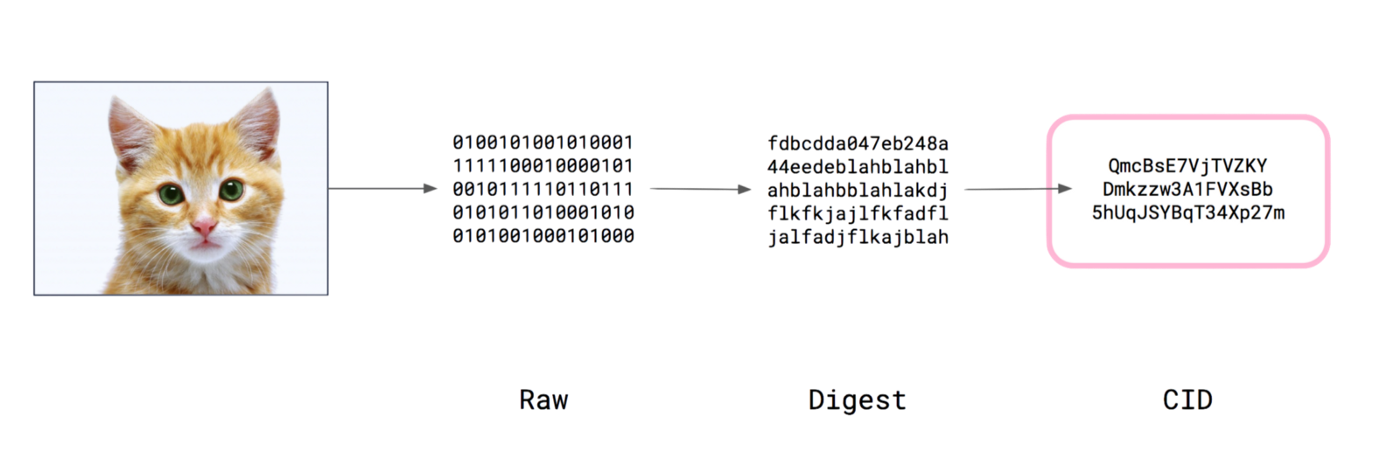
\includegraphics[width=\textwidth]{ipfs_raw_dig_cid_1.png}
        \caption{From raw image to cryptographic digest to content id (multihash).}
        \label{img:ipfsalgorithmvis1}
      \end{subfigure}
      % \hfill
      \begin{subfigure}[!hbtp]{0.45\textwidth}
        \centering
        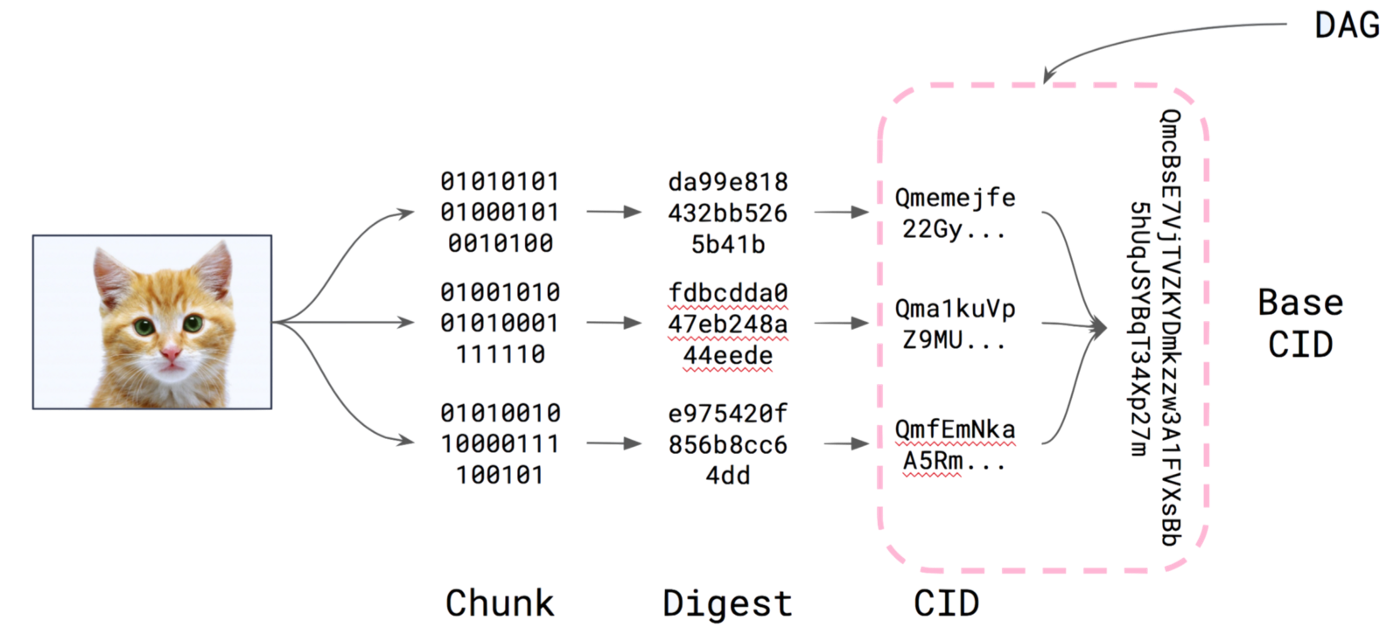
\includegraphics[width=\textwidth]{ipfs_raw_dig_cid_2.png}
        \caption{Large files are chunked, hashed, and organized into an IPLD (Merkle DAG object).}
        \label{img:ipfsalgorithmvis2}
      \end{subfigure}
      \caption{IPFS base CID construction}
      \label{img:ipfsAlgorithmVis}
    \end{figure}
  \end{frame}

  \begin{frame}{What is Blockchain}
    A blockchain is a growing list of records, called blocks, that are securely linked together using cryptography. Each block contains a cryptographic hash of the previous block, a timestamp, and transaction data (generally represented as a Merkle tree, where data nodes are represented by leafs).

    \begin{figure}
      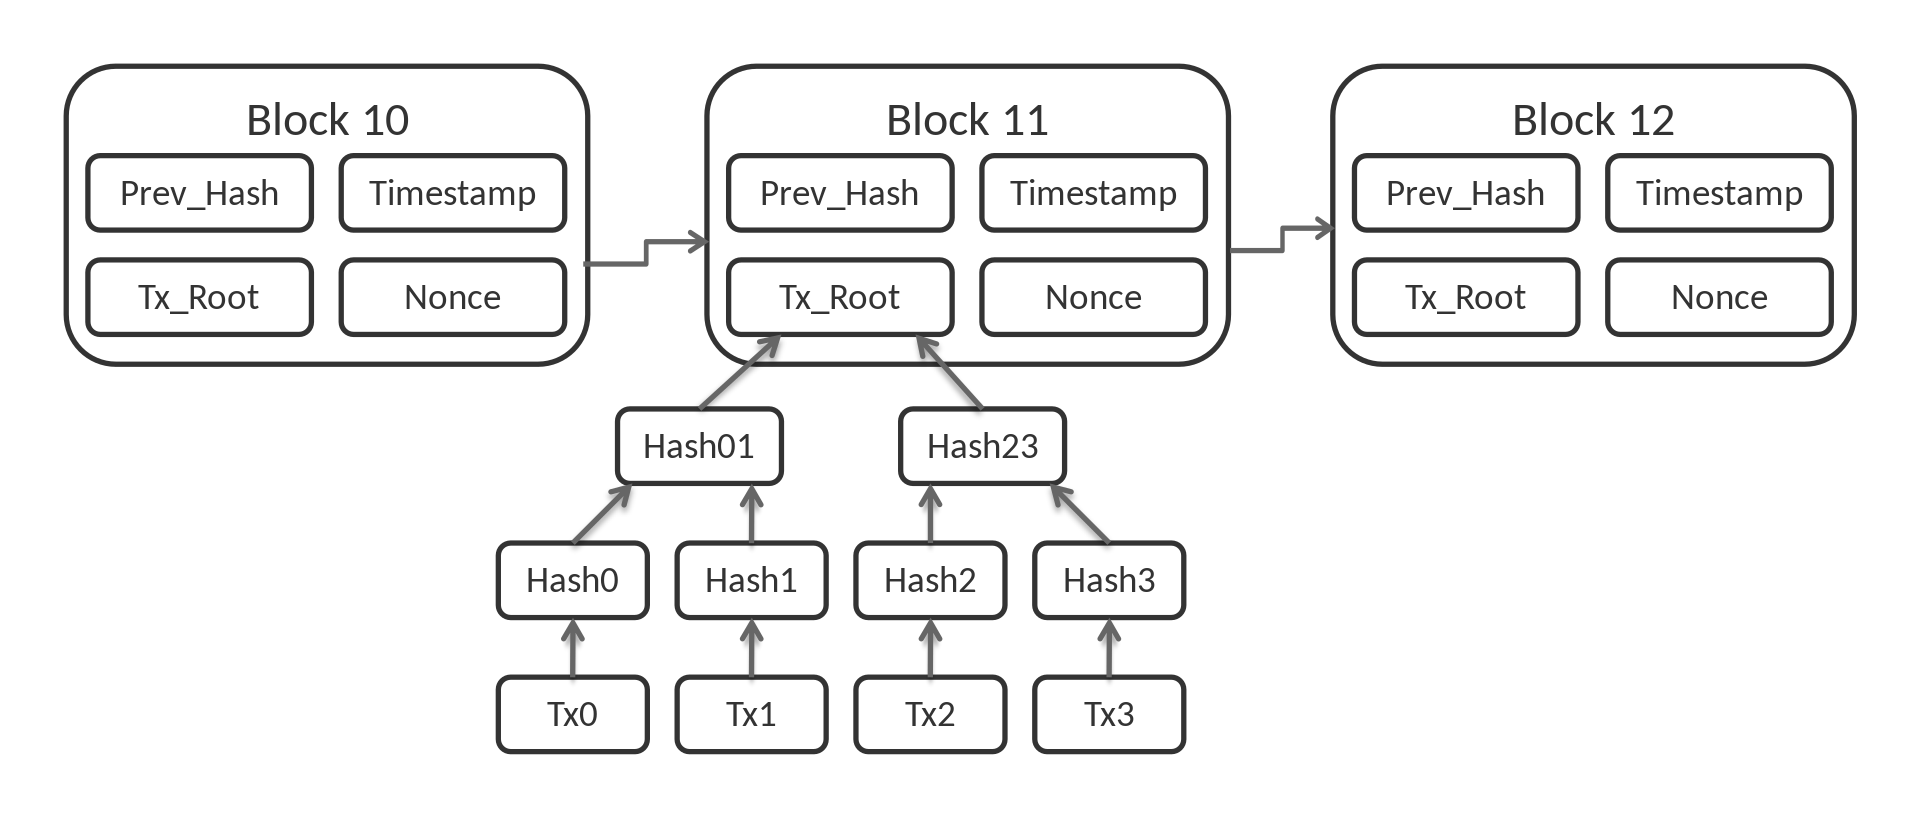
\includegraphics[width=0.7\textwidth]{bitcoin_blockchain_structure.png}
      \caption{Bitcoin blockchain structure.}
    \end{figure}
  \end{frame}

  \begin{frame}{What is a Smart contract}
    A ``smart contract'' is simply a program that runs on the Ethereum blockchain. It's a collection of code (its functions) and data (its state) that resides at a specific address on the Ethereum blockchain.

    Smart contracts are a type of Ethereum account. This means they have a balance and they can send transactions over the network. However they're not controlled by a user, instead they are deployed to the network and run as programmed.
  \end{frame}

  \begin{frame}{Wallet Auth}
    To transact on Ethereum, you need an account. There is no MySQL ``users'' table. There is no email/password login.

    To create an Ethereum account, you need to set up a crypto wallet like Metamask. The wallet will be responsible for generating and securing your crypto keys for signing transactions.

    \begin{figure}
      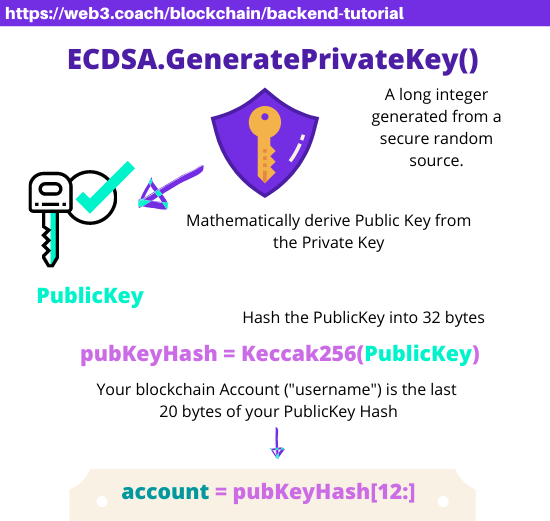
\includegraphics[width=0.25\textwidth]{ecdsa_generate_key.png}
      \caption{Generating keys and addresses.}
    \end{figure}
  \end{frame}

  \section{Methodology}

  \begin{frame}{Development Methodology}
    In this project we use both waterfall and scrum methodologies.
    We used the waterfall methodology for developing the smart contract because we can not update it once we deploy it. And for the rest, we used the scrum methodology.

    \begin{figure}
      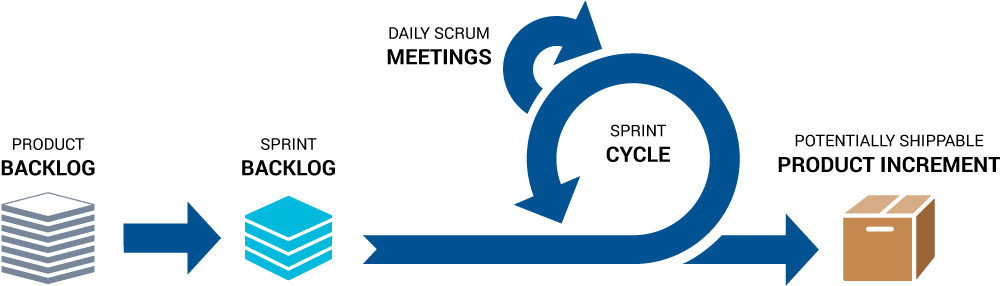
\includegraphics[width=0.8\textwidth]{scrum.png}
      \caption{Agile scrum development process.}
    \end{figure}
  \end{frame}

  \begin{frame}{Use Case Modeling}
    \begin{figure}
      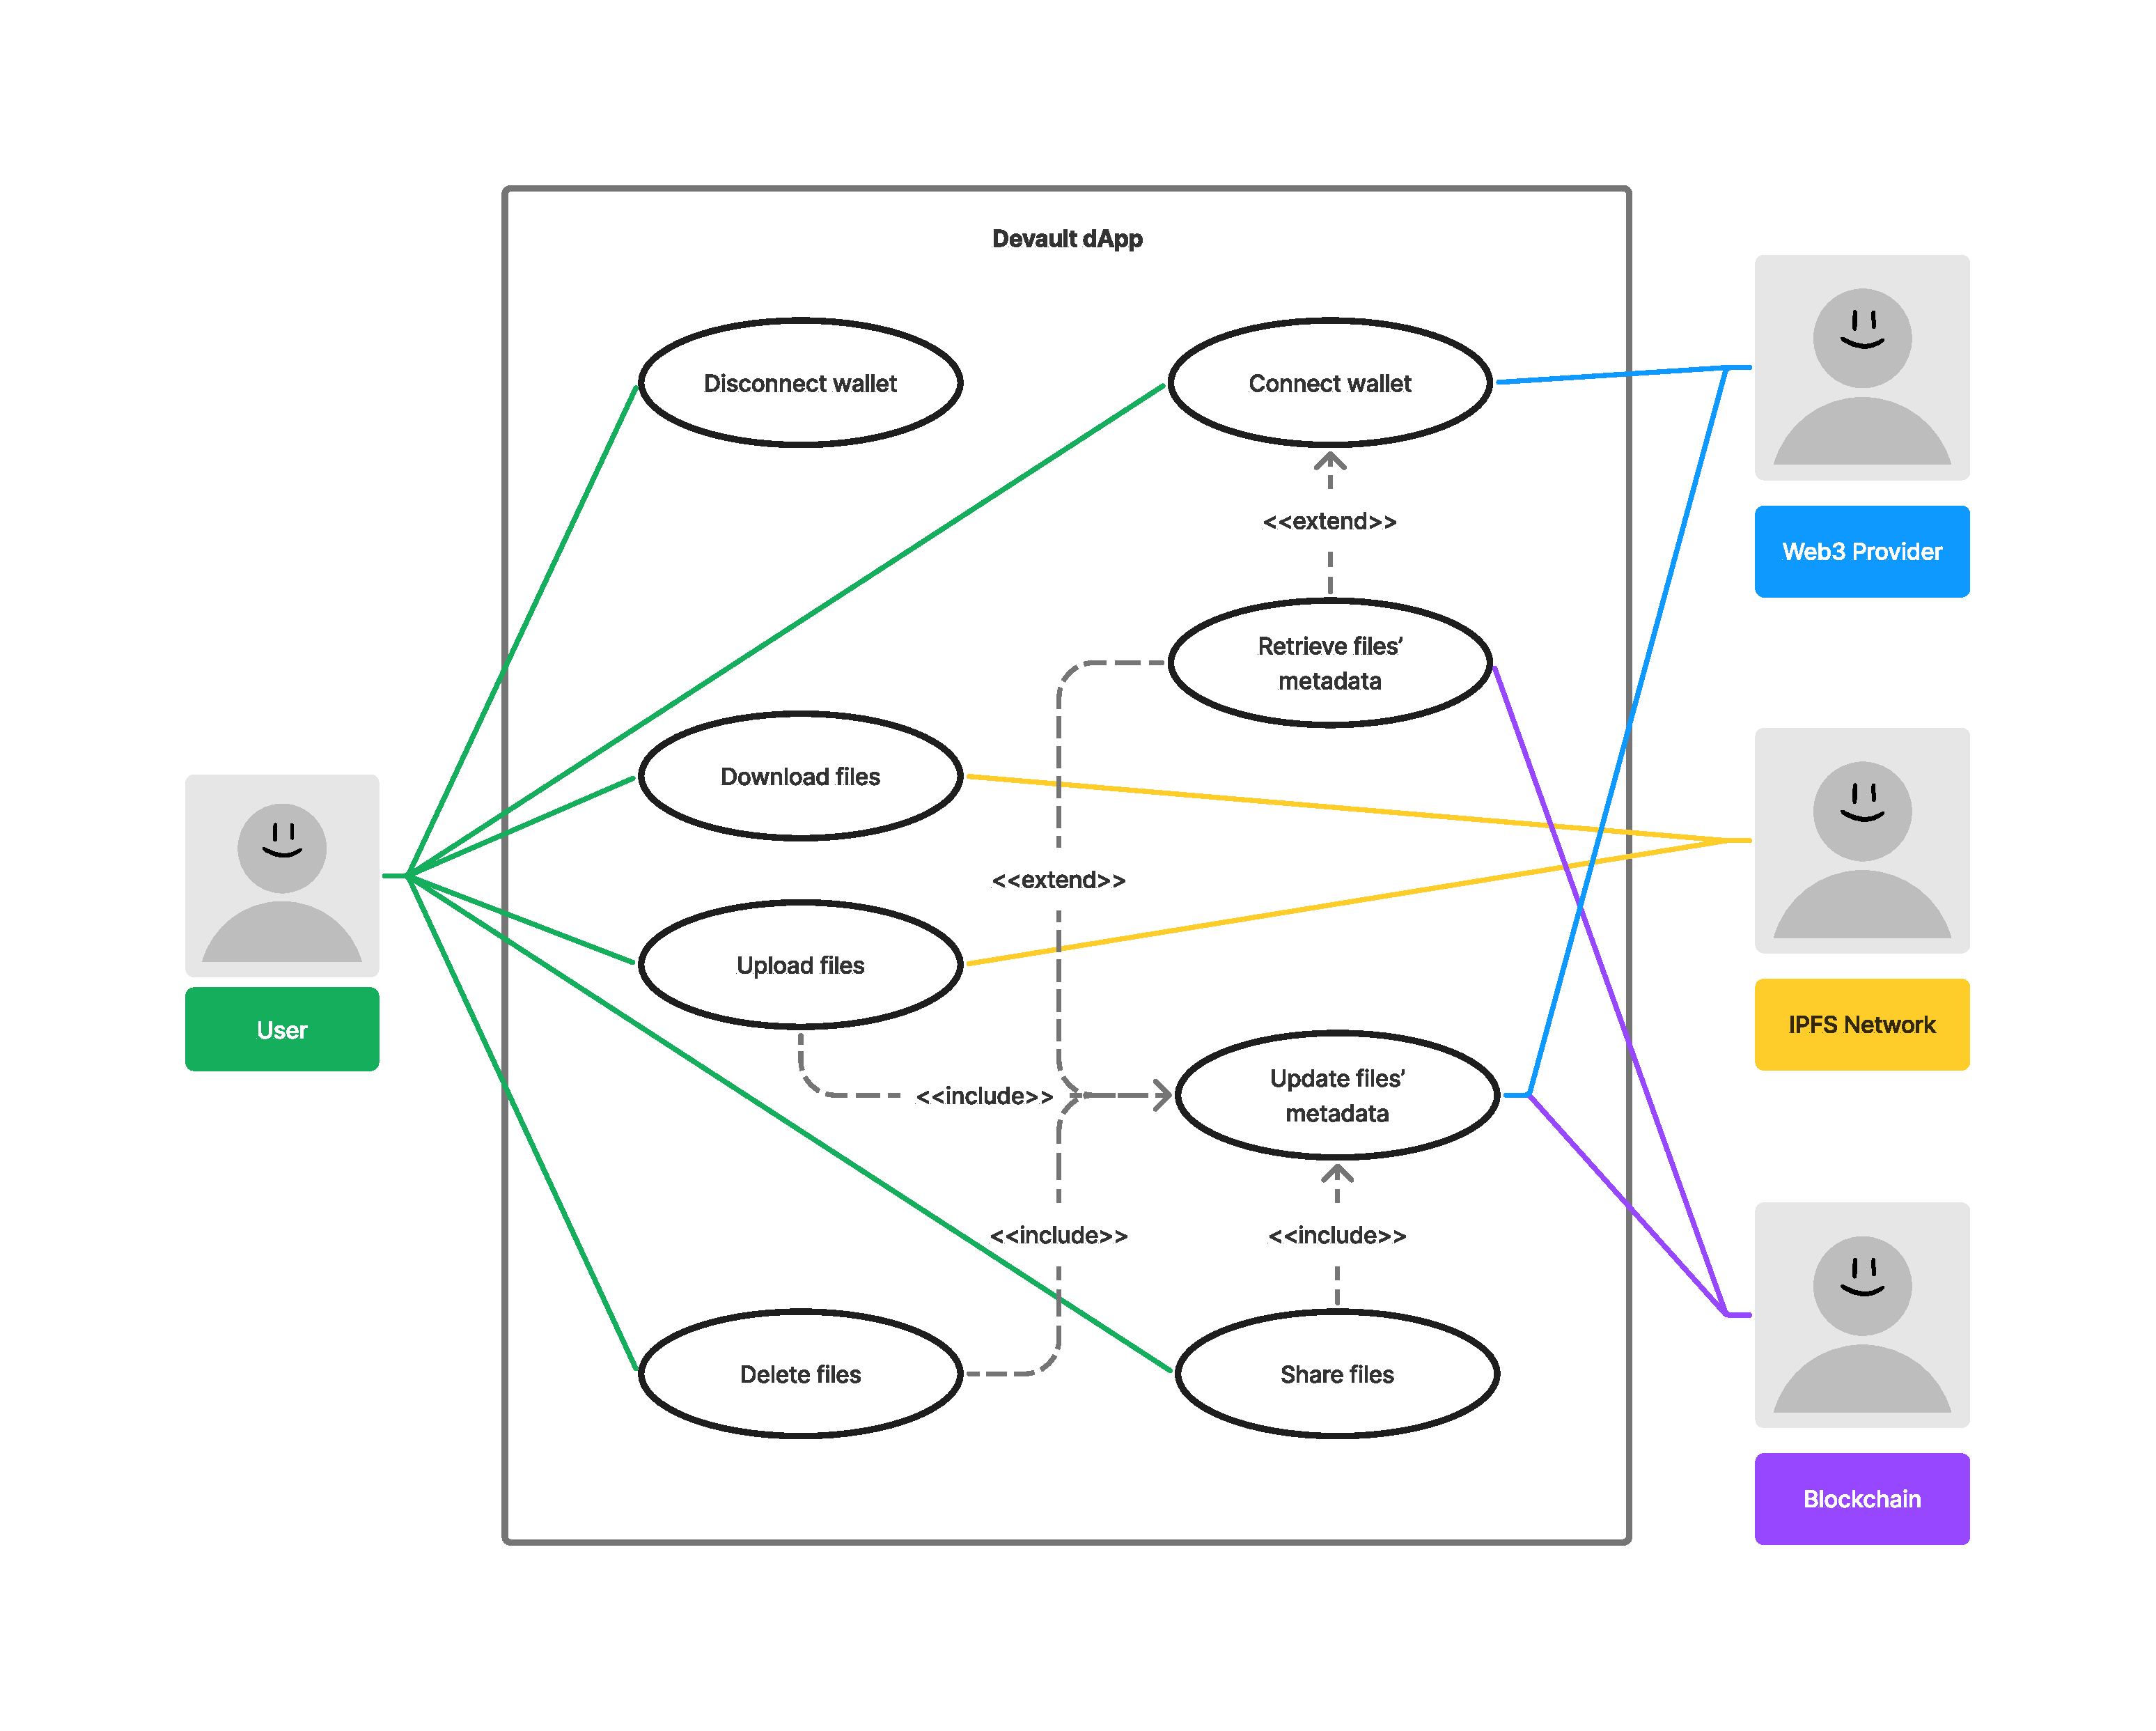
\includegraphics[width=0.5\textwidth]{dapp_uscs_dig.pdf}
      \caption{Devault dApp use case diagram.}
    \end{figure}
  \end{frame}

  \begin{frame}{Sequence Diagram}
    \begin{figure}
      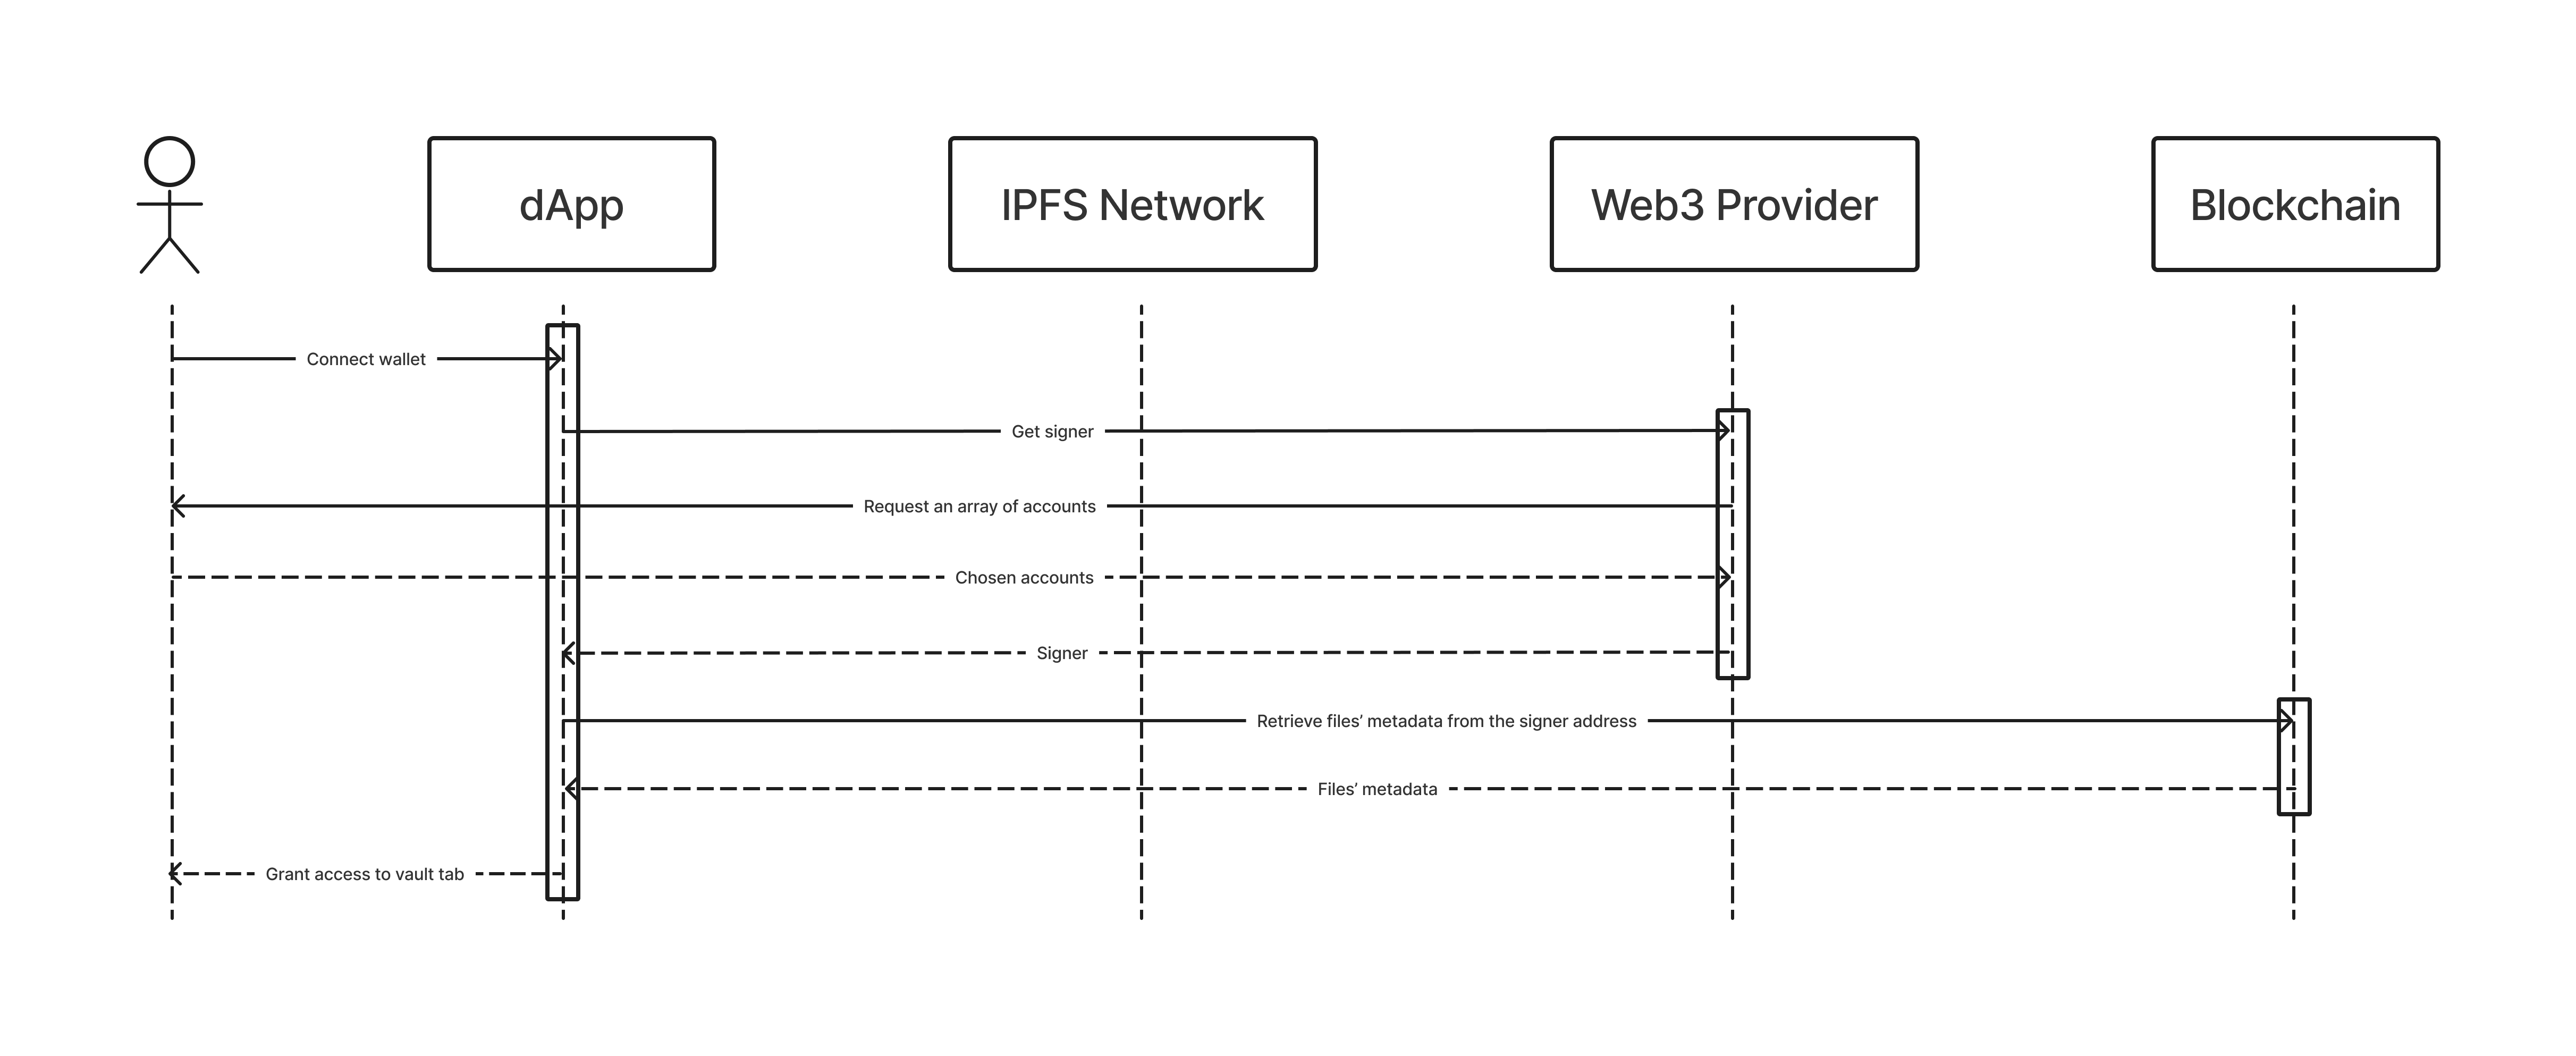
\includegraphics[width=\textwidth]{connect_seq_dig.png}
      \caption{Connect wallet act in sequential order.}
    \end{figure}
  \end{frame}

  \begin{frame}{Sequence Diagram}
    \begin{figure}
      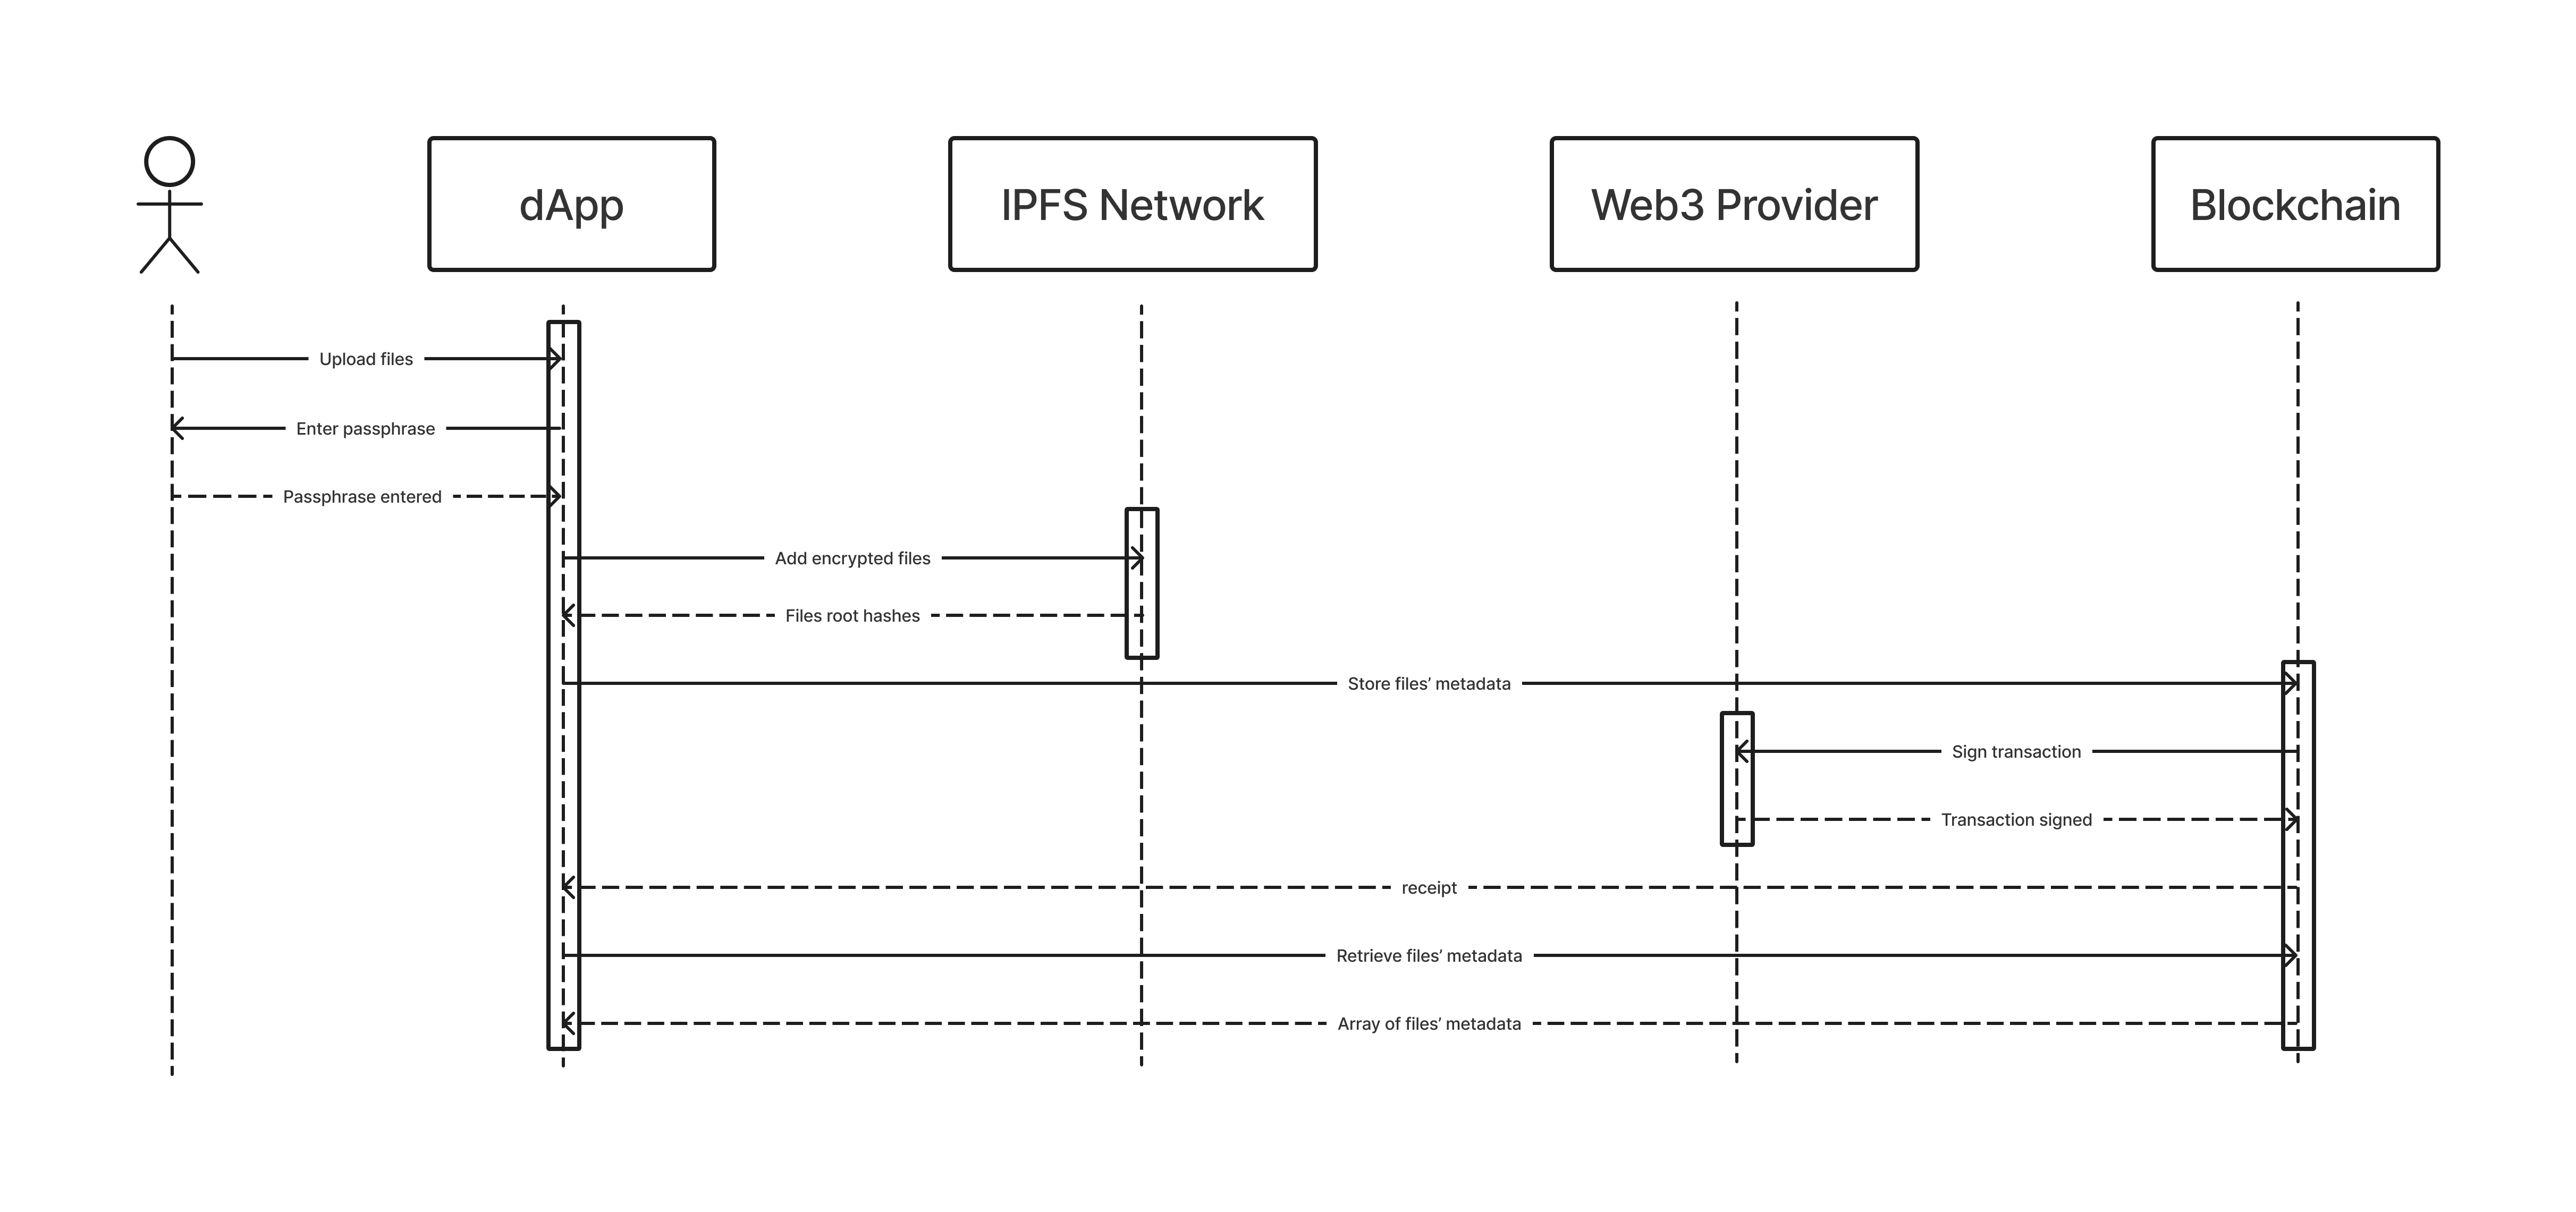
\includegraphics[width=0.9\textwidth]{upload_files_seq_dig.png}
      \caption{Upload files act in sequential order.}
    \end{figure}
  \end{frame}

  \begin{frame}{Sequence Diagram}
    \begin{figure}
      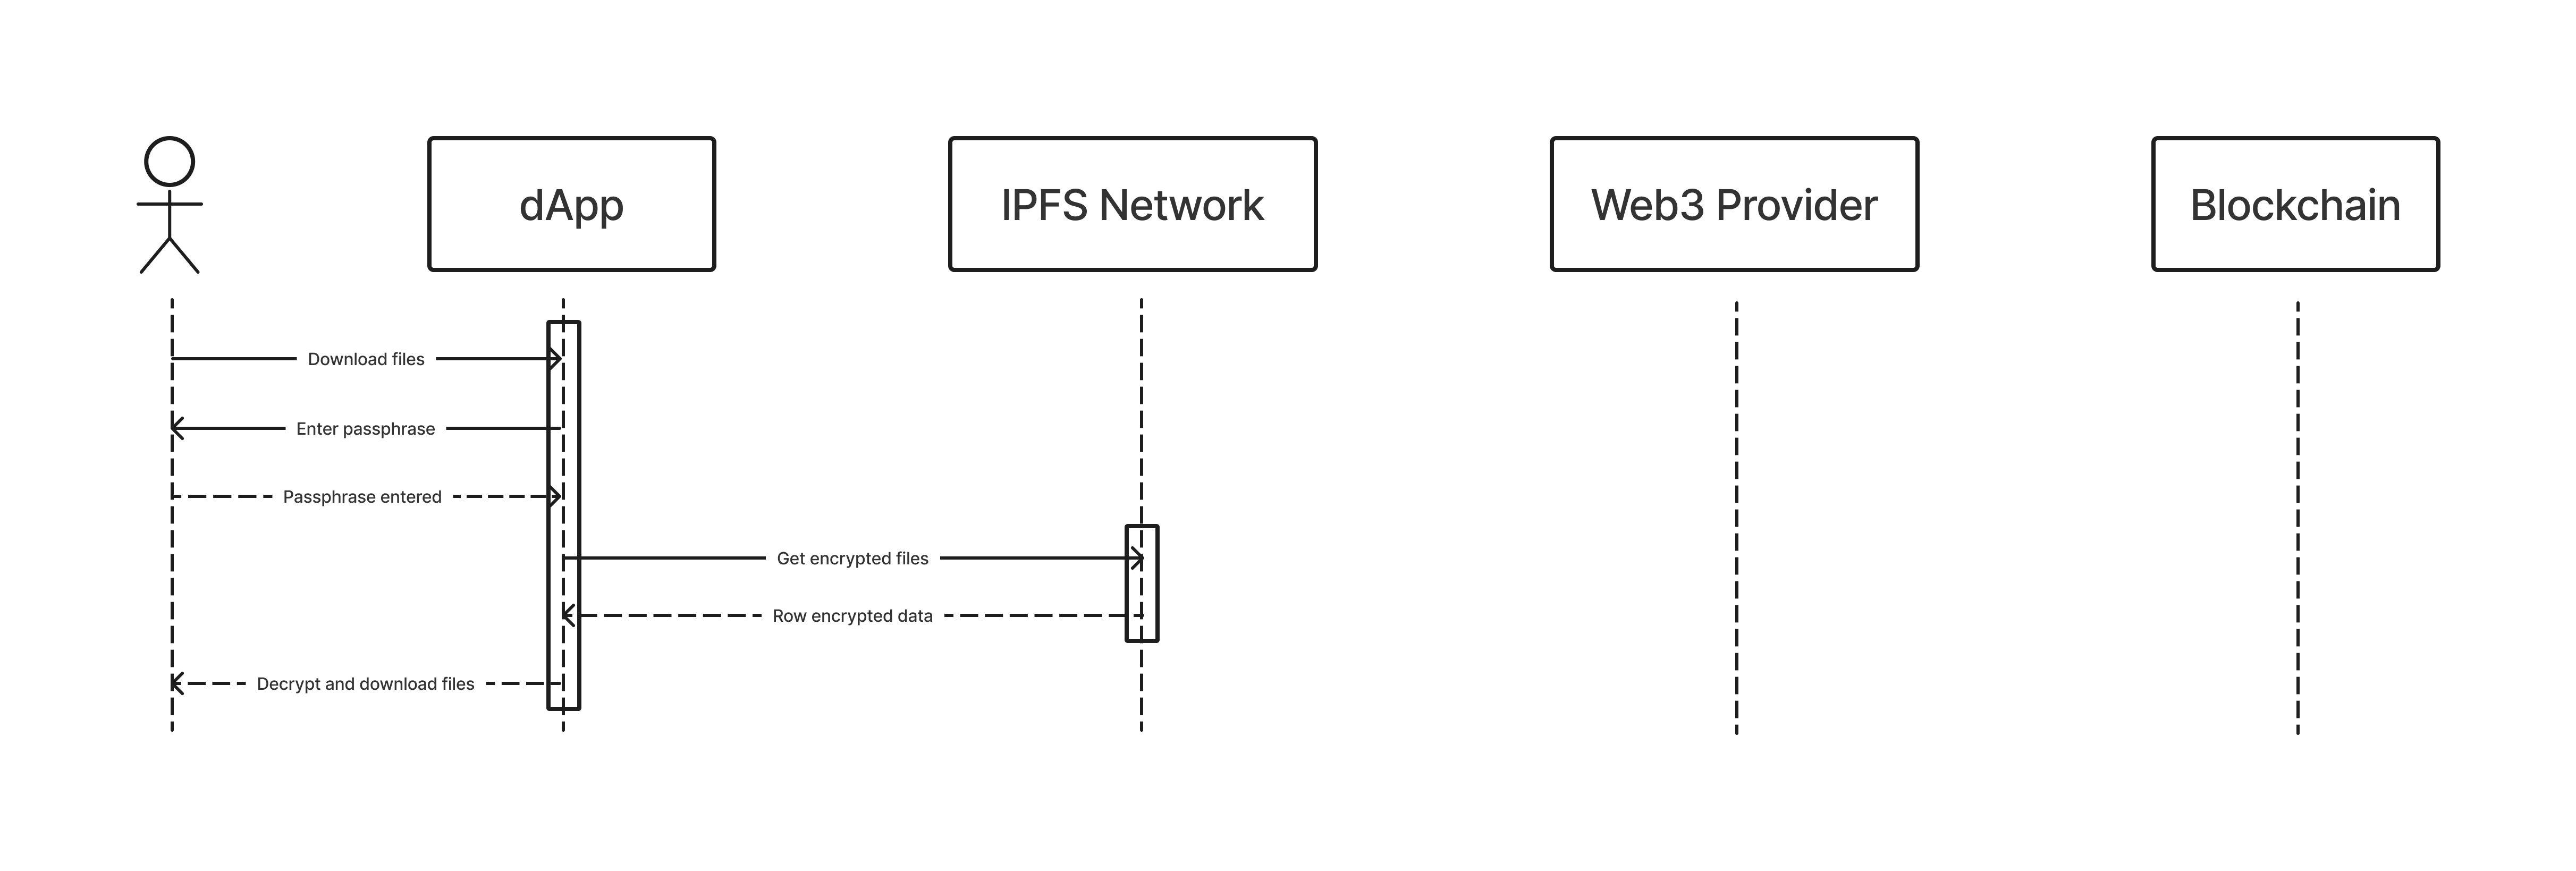
\includegraphics[width=\textwidth]{download_files_seq_dig.png}
      \caption{Download files act in sequential order.}
    \end{figure}
  \end{frame}

  \section{System Design}

  \begin{frame}{System Architecture}
    Here is the conceptual model that defines the structure, behavior, and more views of a system.

    \begin{figure}
      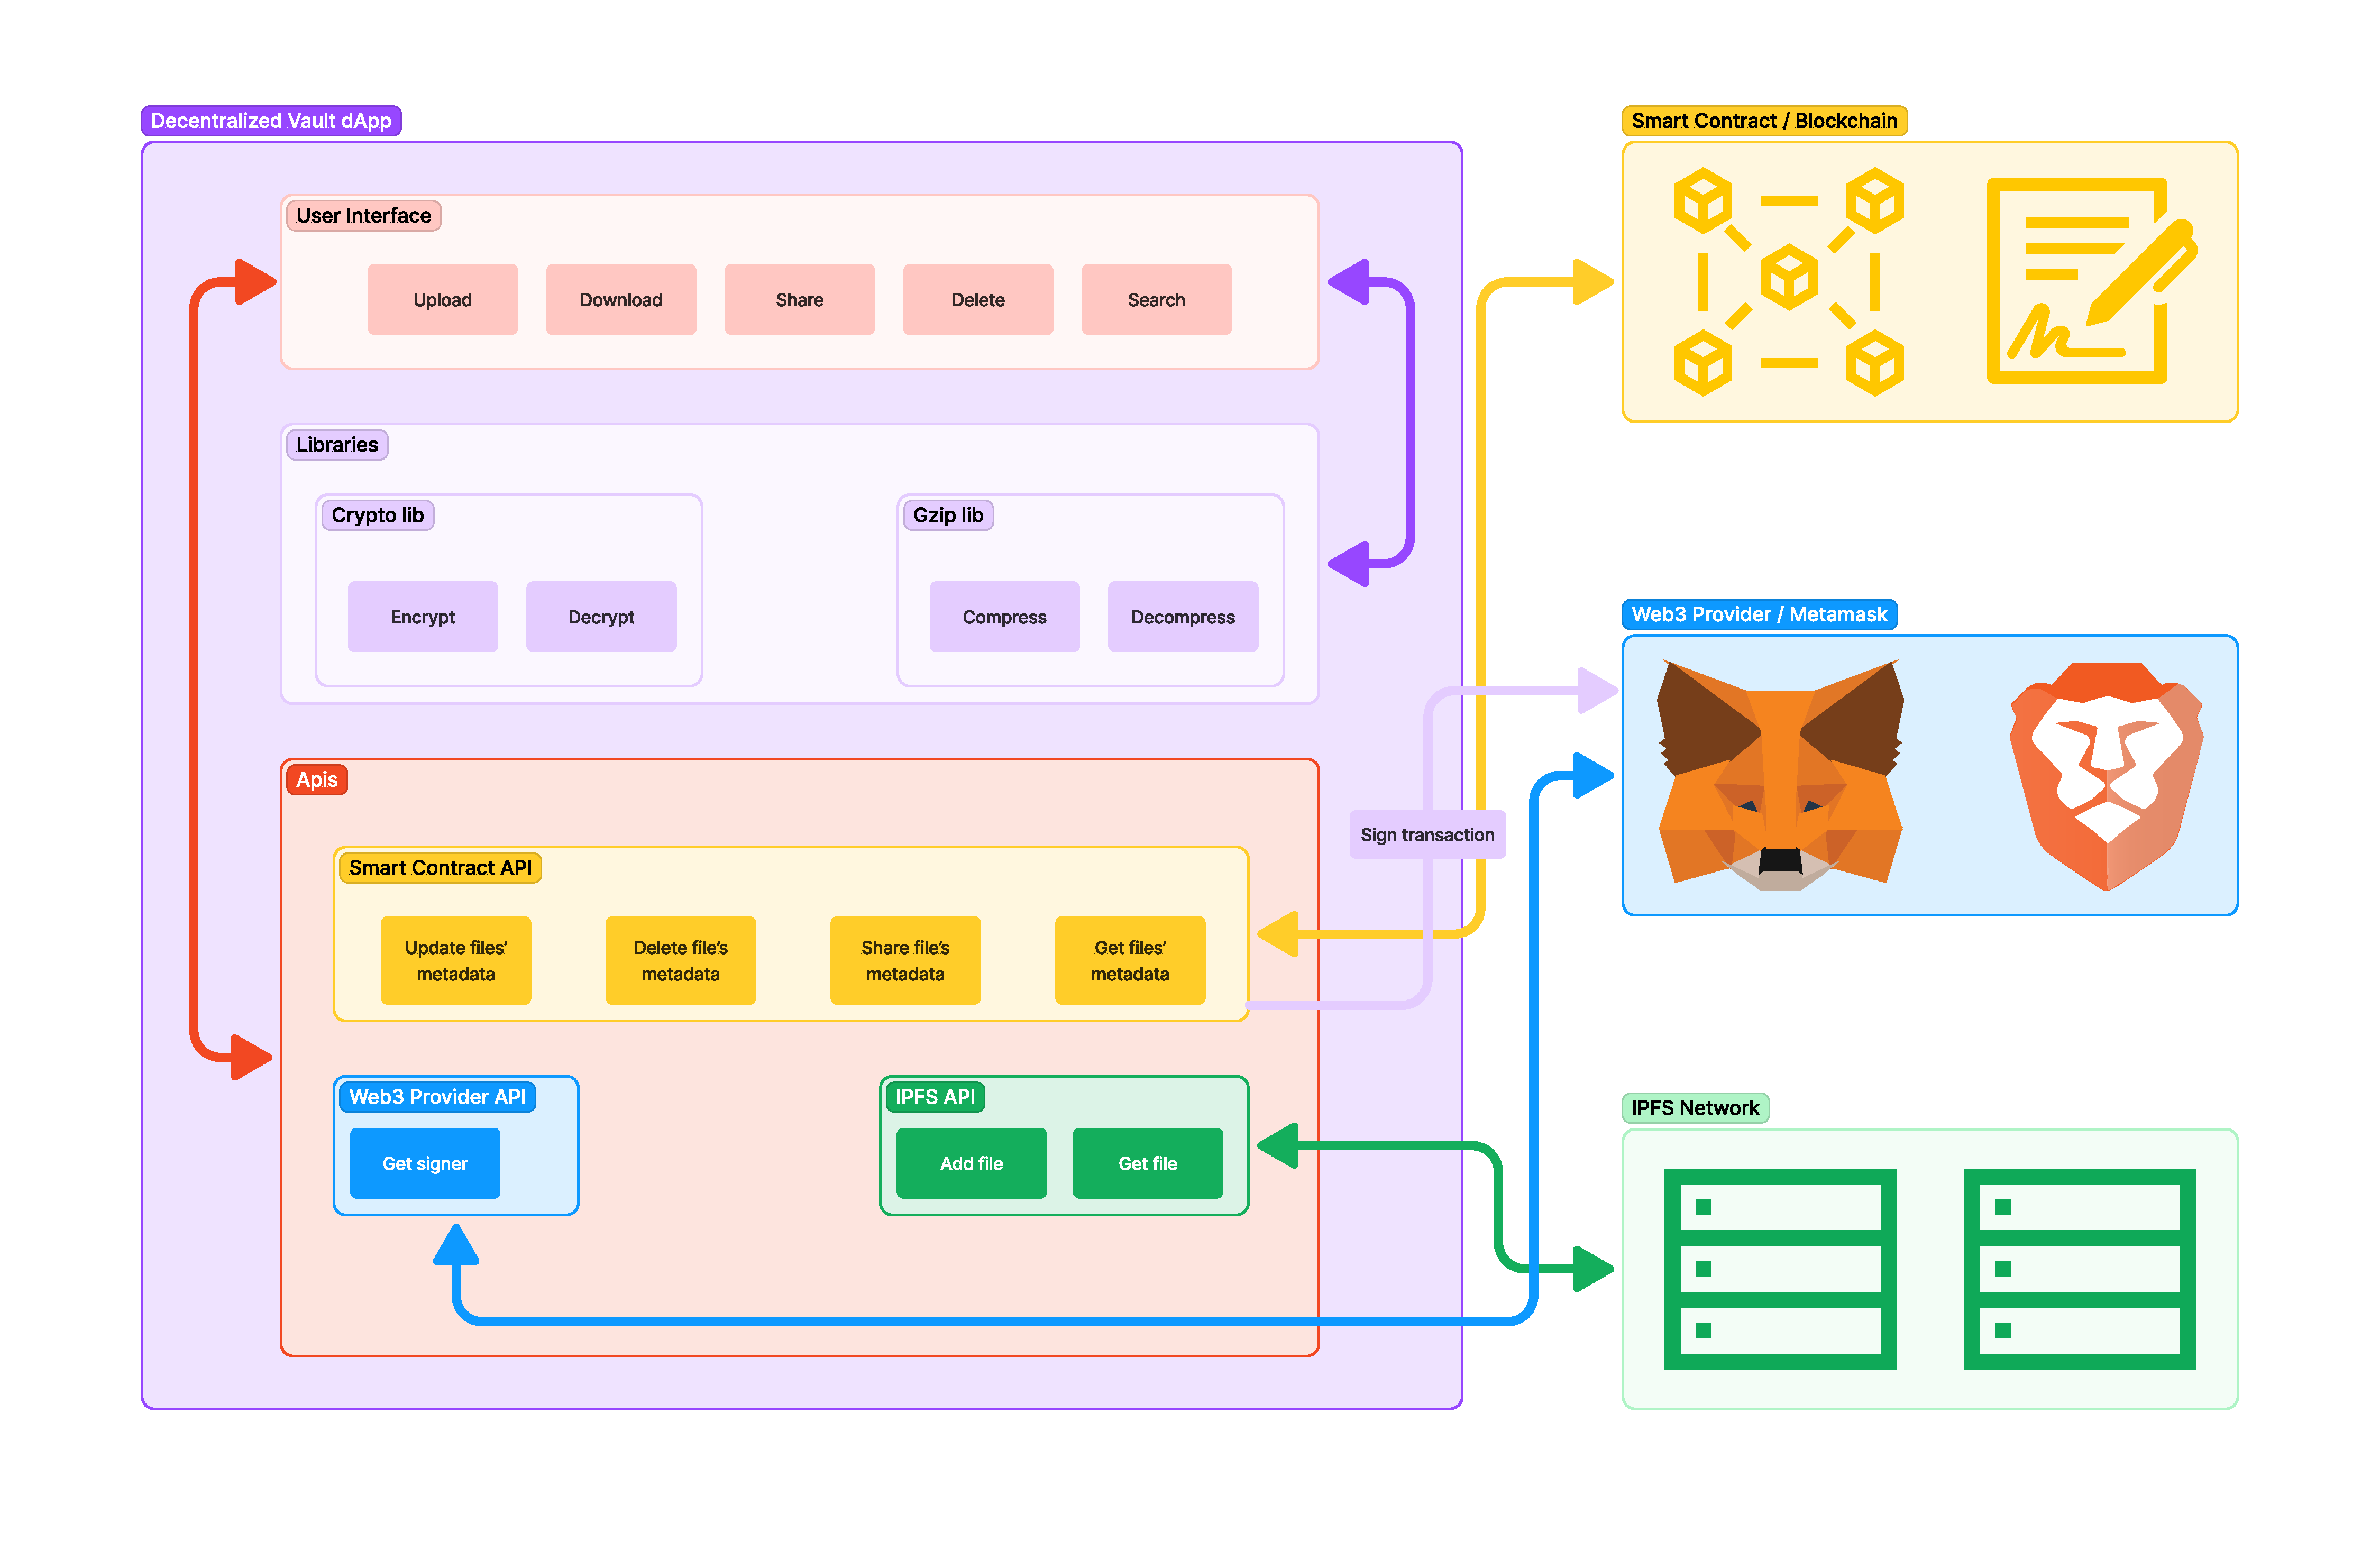
\includegraphics[width=0.5\textwidth]{system_arch.pdf}
      \caption{Decentralized vault dApp architecture.}
    \end{figure}
  \end{frame}

  \begin{frame}{Tools and Technologies}
    \begin{itemize}
      \begin{multicols}{3}
      \item JavaScript
      \item \faReact{} Next.js
      \item Solidity
      \item Hardhat
      \item Ethers.js
      \item Metamask
      \item Infura
      \item IPFS
      \item Etherscan
      \item \faCodeBranch{} GitHub Actions
      \item \faDocker{} Docker
      \item Vercel
      \item Bash/Shell
      \item Emacs
      \item Neovim
      \item Figma
      \item LaTeX
      \end{multicols}
    \end{itemize}
  \end{frame}

  \section{Result and Discussion}

  \begin{frame}{Result}
    We tested the Devault with uploading, downloading, sharing, deleting, connecting, and disconnecting functionality on different browsers and devices. Below we show the results of two of these tests. \\

    \textbf{1. \textit{Brave browser, the desktop version and metamask}} \\

    \begin{figure}
      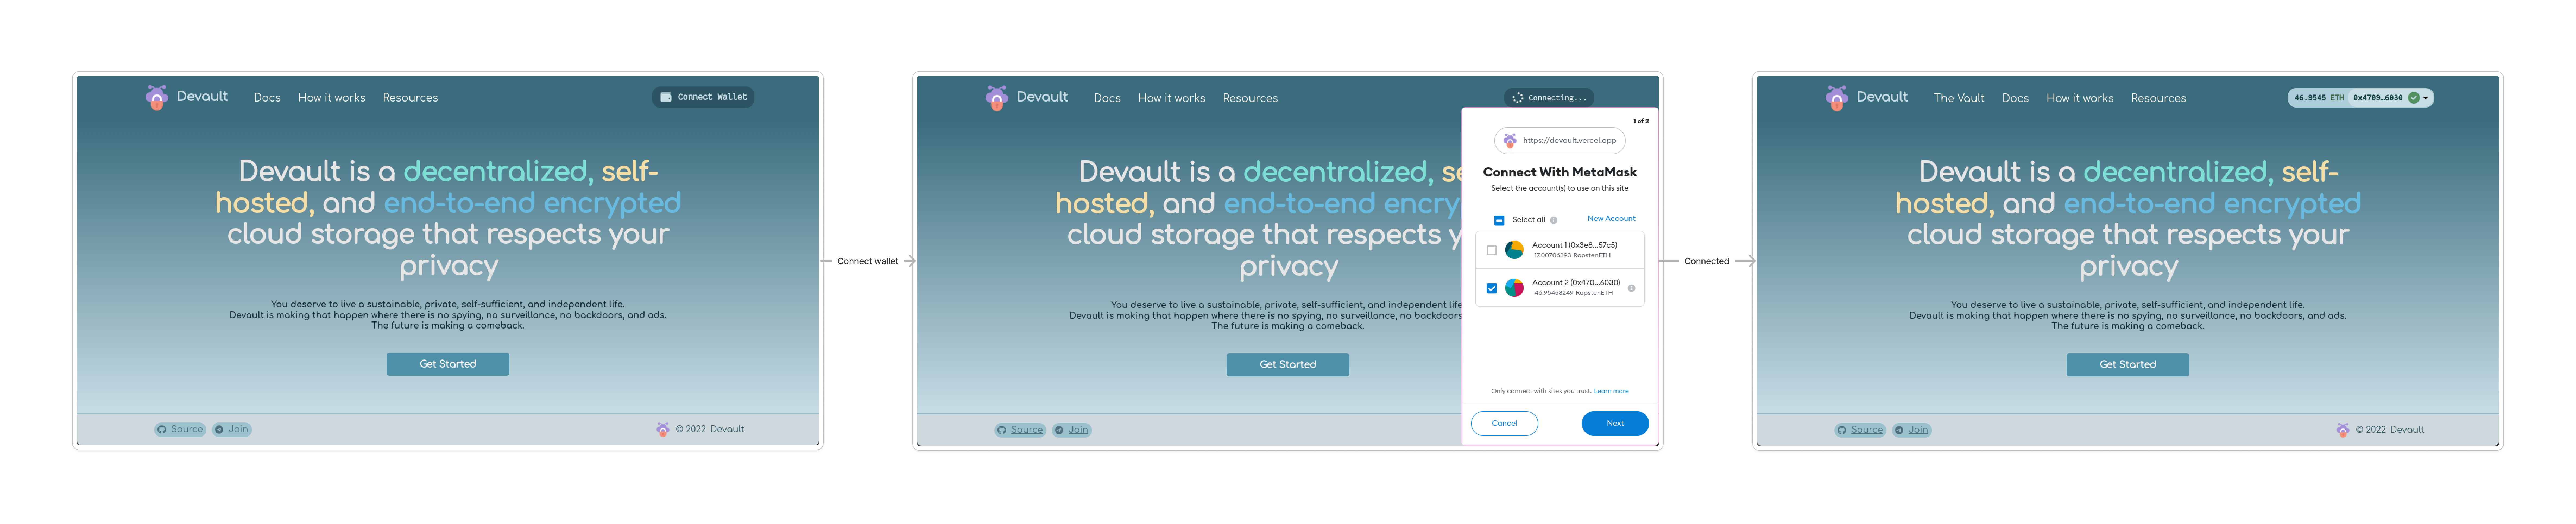
\includegraphics[width=\textwidth]{connect_result.png}
      \caption{The user experience of connecting wallet.}
    \end{figure}
  \end{frame}

  \begin{frame}{Result}
    \textbf{2. \textit{Brave browser, the mobile version and brave wallet}} \\

    \begin{figure}
      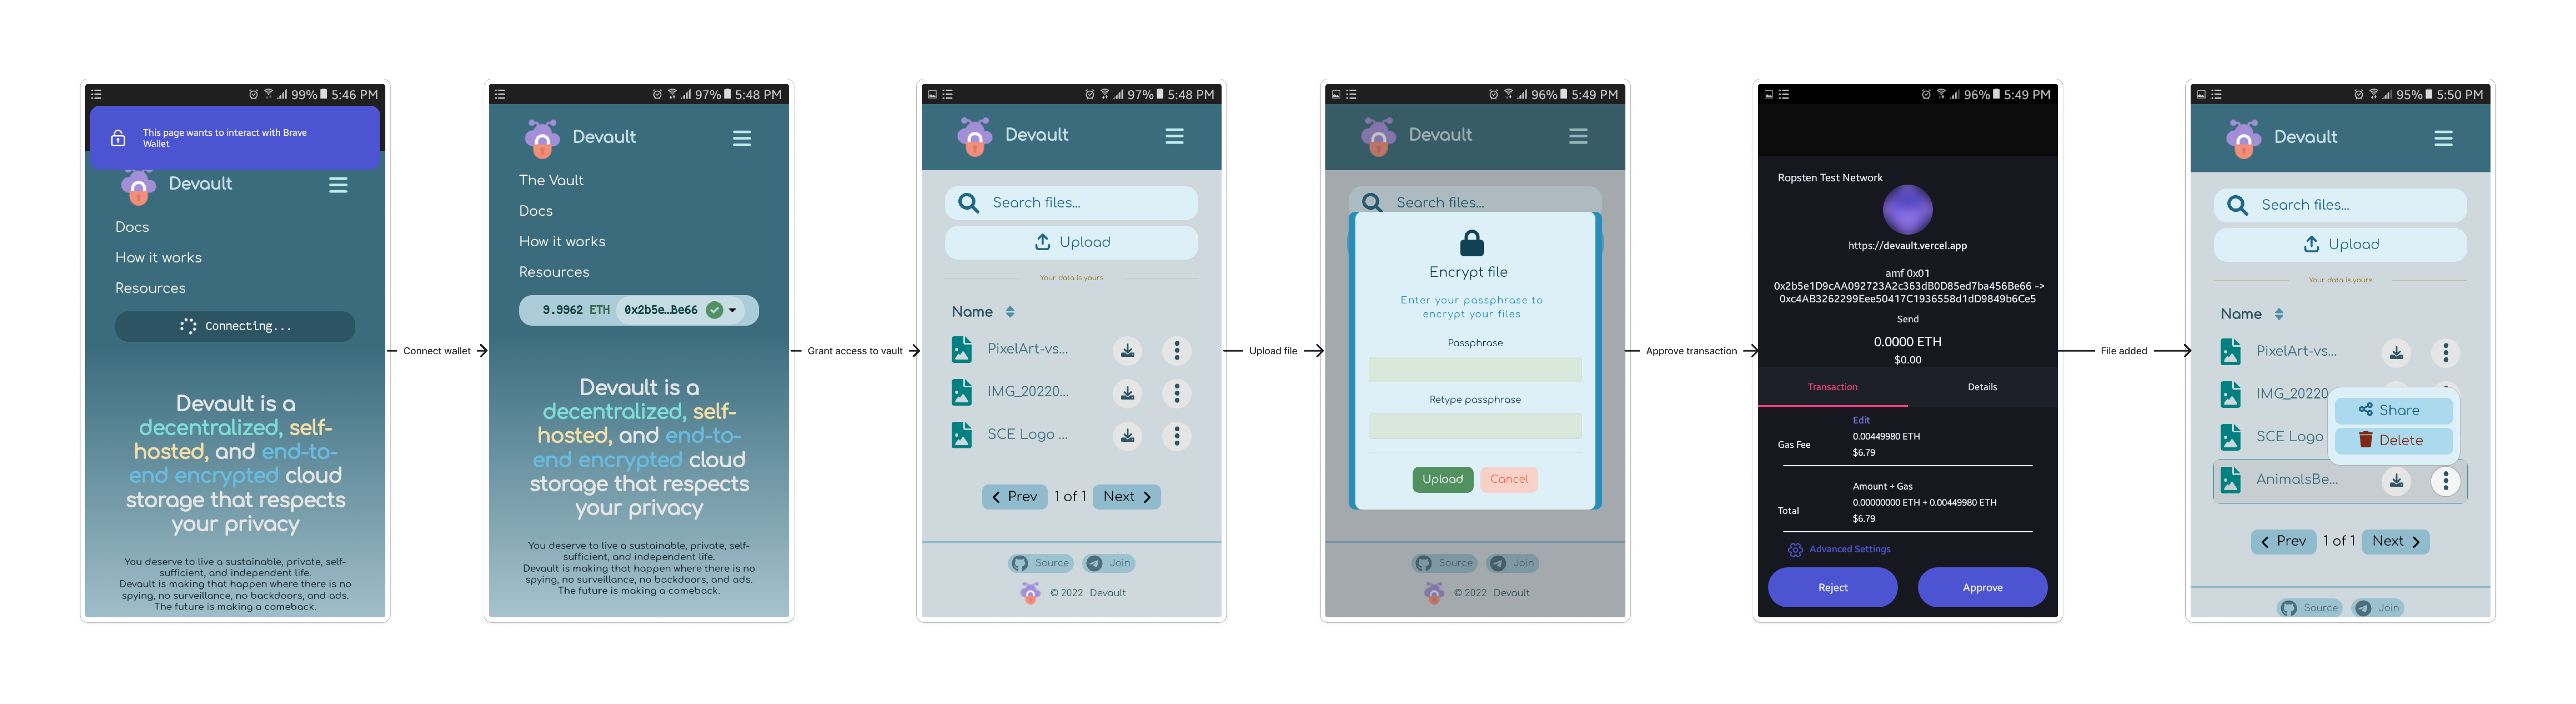
\includegraphics[width=\textwidth]{upload_result.png}
      \caption{The user experience of uploading files.}
    \end{figure}
  \end{frame}

  \begin{frame}{Limitation}
    The limitations of our system are listed below: \\[8pt]

    \begin{itemize}
    \item The user should have cryptocurrency to make transactions and to reward the entity for renting their hard disk, which is a constraint.
    \item The user should install specific software such as metamask or brave wallet to use our system.
    \item Cryptocurrencies are illegal in some countries, whereas our system needs those cryptocurrencies to work.
    \item The uploading of a file may take a while because of the encryption and block mining, which is not practical.
    \end{itemize}
  \end{frame}

  \begin{frame}{Future Work}
    The limitations of our system are listed below: \\[8pt]

    \begin{enumerate}
    \item Support Arabic language.
    \item Use Shamir's Secret Sharing algorithms for sharing files.
    \item Add the search functionality.
    \item Compress files before uploading.
    \item Enhance the ui/ux.
    \item Manipulate selected files and folders.
    \item Deploy to the mainnet.
    \item Use Filecoin instead of IPFS.
    \item Use the advantages of private and public keys in encryption/decryption.
    \item Give feedback if the key used for decryption is not the same key used for encryption.
    \end{enumerate}
  \end{frame}

	\begin{frame}[standout]
		Demo
	\end{frame}

	\begin{frame}[allowframebreaks]{References}
    \nocite{*}
    \bibliography{resources/bibliography}
		\bibliographystyle{unsrt}
	\end{frame}

\end{document}
